\documentclass[11pt,a4paper]{article}

\usepackage[utf8]{inputenc}
\usepackage[T1]{fontenc}
\usepackage{lmodern}
\usepackage[margin=2.5cm]{geometry}
\usepackage{graphicx}
\usepackage{booktabs}
\usepackage{amsmath}
\usepackage{amssymb}
\usepackage{siunitx}
\usepackage{caption}
\usepackage{subcaption}
\usepackage{float}
\usepackage{enumitem}
\usepackage[hidelinks]{hyperref}
\usepackage{xcolor}

\graphicspath{{results/plots/eda/}{results/plots/phase1/}{results/plots/phase2/}{results/plots/phase3/}}

\captionsetup{font=small,labelfont=bf}
\setlength{\parskip}{0.4em}
\setlength{\parindent}{0pt}

\title{\bfseries Operational State Recognition and Braking Behavior\\
Analysis for Predictive Maintenance on Metro Trains\\[0.4em]
\large Project Report --- Phases~1--3}

\author{Maximilian Scheiblauer (11776651)\\[0.3em]
\small Domain Lecture: 330.331 Instandhaltungsmanagement, TU Wien\\
\small Domain Supervisor: Dr.~Andreas Steiner \quad Data Science Supervisor: Dr.~Florina Piroi}

\date{4 June 2026}

\begin{document}

\maketitle

\begin{abstract}
\noindent\small
Urban metro systems are still maintained on fixed time- or mileage-based intervals,
which ignore how a vehicle is actually operated and so cause both premature part
replacement and unexpected, service-disrupting failures. This report develops data-driven
maintenance indicators from MetroAT --- a one-year, 1\,Hz, 109-signal pneumatic-system
dataset from a single Wiener Linien metro train, enriched with documented failure and
maintenance events --- following the CRISP-DM process. Phase~1 recovers operational regimes
by unsupervised learning and validates them against documented events; Phase~2 isolates
individual braking events, classifies their intensity, and tests for pre-failure
degradation trends; Phase~3 extends the work beyond the original proposal with an
out-of-sample test, degradation localization, a multivariate health index, and an explicit
failure forecaster. The headline results are three transferable operational regimes
(adjusted Rand index 0.97 from pneumatics alone; structure stable out-of-sample), a
reproducible dataset of 157{,}823 braking events, degradation localized to a brake-cylinder
sensor in the week of a documented brake failure, a multivariate health index detecting
30\,\% of failures at a 15.3-day mean lead with zero false alarms, and a weak-but-real
7-day failure forecast whose strongest drivers coincide with that health index. The binding
constraint throughout is data, not method: every failure-related claim rests on ten
flag-derived failures on one train, so the honest deliverable is a validated pipeline and a
clear statement of what additional data would make it operationally deployable.
\end{abstract}

\setcounter{section}{0}
\section{Introduction}
\label{sec:intro}

\subsection{Motivation}
Metro operators schedule maintenance on fixed time- or mileage-based intervals. Such
schedules treat every vehicle and every operating day as equivalent, even though wear is
driven by how a train is actually used --- its braking behaviour, route profile, and load.
The consequence is twofold inefficiency: components are replaced before they are worn out,
and others fail unexpectedly between scheduled services, causing costly disruption.
Condition-based (predictive) maintenance aims to close this gap by deriving wear indicators
directly from on-board sensor data. The pneumatic subsystem is a compelling first target:
it accounts for roughly 20\,\% of metro failures and contains safety-critical components
--- the service and parking brakes, the air-suspension levelling system, and the
air-production (compressor) unit.

\subsection{Problem statement}
This project addresses three problems. \textbf{P1 (Maintenance impact assessment):}
operational variability affects component wear, but maintenance schedules do not
distinguish high-wear from normal operation. \textbf{P2 (Braking degradation):} braking is
the primary contributor to mechanical wear, and quantifying braking intensity and detecting
its degradation could enable targeted intervention. Both are taken verbatim from the project
exposé. Phase~3 then adds \textbf{P3 (Localization and forecasting, an extension):} can
degradation be \emph{localized} to a component and failures \emph{forecast} from the same
signals?

\subsection{Research questions and expected outcomes}
The exposé poses four research questions (RQ1--RQ4) with paired outcomes (O1--O4); Phase~3
adds five further questions (RQ5--RQ9). Table~\ref{tab:rqs} maps each to the section that
answers it.

\begin{table}[H]
\centering
\caption{Research questions, phases, and the sections that address them.}
\label{tab:rqs}
\small
\begin{tabular}{l p{10.0cm} l}
\toprule
ID & Question / outcome & Section\\
\midrule
RQ1/O1 & Can distinct operational regimes be identified, with transition structure? & \ref{sec:phase1}\\
RQ2/O2 & Which features associate most strongly with the regimes (and maintenance)? & \ref{sec:phase1}\\
RQ3/O3 & Are there temporal patterns in braking intensity? Build a labelled event set. & \ref{sec:phase2}\\
RQ4/O4 & Can degradation trends be detected before documented brake failures? & \ref{sec:phase2}\\
RQ5 & Do the pneumatic sensors recover the regimes without the velocity channel? & \ref{sec:phase3}\\
RQ6 & Which sensor groups drive the variance the clustering sees? & \ref{sec:phase3}\\
RQ7 & Can degradation be localized to a specific wagon/bogie component? & \ref{sec:phase3}\\
RQ8 & Does a multivariate health index detect failures with usable lead time? & \ref{sec:phase3}\\
RQ9 & Can failures be forecast over a fixed horizon, and what are the drivers? & \ref{sec:phase3}\\
\bottomrule
\end{tabular}
\end{table}

\subsection{Contributions}
The project contributes: (i) a methodology for recovering maintenance-relevant operational
regimes from multivariate pneumatic sensor data, validated against documented events;
(ii) a reproducible braking-event dataset with an interpretable intensity classifier;
(iii) a frozen-model, out-of-sample demonstration that the regimes transfer to unseen
months; (iv) a multivariate pneumatic health index that localizes degradation and detects
failures with real lead time; (v) a horizon-classification failure forecaster with SHAP
driver analysis; and (vi) an open, streaming, fully reproducible analysis pipeline. A
cross-cutting contribution is an honest characterisation of the dataset's binding limit
--- ten flag-derived failures on one train --- and a concrete plan for what data would lift it.

\subsection{Report structure}
Section~\ref{sec:background} gives background and positions the methods. Section~\ref{sec:data}
covers data understanding, including the deviations between the delivered data and the
exposé. Section~\ref{sec:method} describes the shared pipeline and the Phase~3 methods.
Sections~\ref{sec:phase1}--\ref{sec:phase3} report Phases~1--3. Section~\ref{sec:discussion}
draws cross-cutting conclusions, Section~\ref{sec:limitations} states the limitations,
Section~\ref{sec:conclusion} concludes with the status of each research question and future
work, and Section~\ref{sec:repro} documents reproducibility.

\setcounter{section}{1}
\section{Background and Related Context}
\label{sec:background}

\subsection{Predictive maintenance for rolling stock}
Urban metro operators traditionally service rolling stock on fixed time- or
mileage-based intervals. Such schedules ignore how a vehicle is actually operated:
two trains with identical mileage can accumulate very different wear depending on their
braking behaviour, route profile, and load. Predictive (condition-based) maintenance
aims to close this gap by deriving wear indicators directly from on-board sensor data,
so that intervention is driven by observed condition rather than by the calendar. The
pneumatic subsystem is a natural first target: it accounts for roughly 20\,\% of metro
failures and contains safety-critical components --- service and parking brakes, the
air-suspension levelling system, and the air-production (compressor) unit.

\subsection{The pneumatic subsystem in the MetroAT train}
The signals analysed here describe the pneumatic brake and air-supply chain. The
relevant component groups are the \emph{proportional valves} (which meter brake
pressure), the \emph{brake cylinders} (which apply the service brake), the
\emph{spring brakes} (parking/holding brake), the \emph{pneumatic braking force}
delivered per bogie, the \emph{main reservoir} (stored compressed air), the
\emph{load pressure} and air-suspension bellows (levelling), and the
\emph{energy-braking resistance}. Each signal is replicated across six wagons and two
bogies per wagon, which is the source of the heavy sensor redundancy documented in
Section~\ref{sec:data}.

\subsection{CRISP-DM and unsupervised regime discovery}
The project follows the CRISP-DM process model, adapted for exploratory time-series
sensor analytics with explicit validation against documented maintenance outcomes.
Phase~1 uses \emph{unsupervised regime discovery}: standardisation, dimensionality
reduction by principal-component analysis (PCA), and $k$-means clustering of short
sensor windows into operational states. Phase~2 builds \emph{event-level features} on
top of those states and applies interpretable intensity classification together with
classical trend and change-point analysis (OLS slope tests, CUSUM) to look for
pre-failure degradation. These methods are deliberately simple and interpretable, which
matters in a maintenance context where category boundaries and alarms must be
explainable to domain experts.

\subsection{Anomaly scoring, change-point detection, and horizon classification}
Phase~3 extends the analysis beyond the exposé and draws on three further families of
methods. \emph{Anomaly scoring} measures how far a window departs from healthy
behaviour: PCA \emph{reconstruction error} captures variance the regime model does not
explain, while the \emph{Mahalanobis distance} measures departure, in correlation-aware
units, from a healthy reference distribution. \emph{Change-point detection} (CUSUM)
turns a noisy health signal into discrete alarms by accumulating deviations until a
tuned threshold is crossed. Finally, \emph{horizon classification} frames failure
forecasting as a supervised problem --- each day is labelled ``failure within $H$ days''
--- evaluated under leave-one-failure-out cross-validation and interpreted with SHAP
feature attributions. These position Phase~3 as the move from \emph{describing} regimes
to \emph{detecting} and \emph{forecasting} degradation.

\setcounter{section}{2}
\section{Data and CRISP-DM Data Understanding}
\label{sec:data}

\subsection{Dataset overview}
MetroAT provides sensor recordings from one Wiener Linien metro train sampled at 1\,Hz.
The data are delivered as Hive-partitioned Parquet (\texttt{year=/month=/day=/day.parquet}).
For this work the year is split into a \textbf{training set} (1~Jun~2024 --- 11~Feb~2025;
246 daily files, \textbf{14{,}342{,}361 rows}) and a held-out \textbf{test set}
(12~Feb~--~Jun~2025) that was sealed and not touched during Phase~1 and Phase~2. All
modelling, threshold setting, and validation in Phases~1 and~2 use the training set
only; the test set is opened for the first time in Phase~3 (Section~\ref{sec:phase3}) as
the project's single genuine out-of-sample check. The test period is failure-rich,
containing \textbf{12 failures and 9 maintenance} events --- a windfall that later makes
an out-of-sample evaluation of the failure forecaster possible at all.

\subsection{Schema}
The confirmed schema has \textbf{109 columns}: 74 continuous sensor signals, 20 binary
signals, 7 operational-state variables, 4 failure/maintenance fields, and 4 timestamp
fields. Continuous signals follow a per-wagon naming convention
\texttt{\{CW1,CW2,MW1..MW4\}\_<signal>\_\{BOGIE1,BOGIE2\}} (six wagons $\times$ two
bogies). The operational-state variables (manual/automatic/emergency mode, brake signal,
line, section, special-section flag) and the four failure/maintenance fields
(\texttt{TRAIN\_IS\_IN\_FAILURE}, \texttt{TRAIN\_IS\_IN\_MAINTENANCE},
\texttt{TRAIN\_FAILURE\_TYPE}, \texttt{TRAIN\_MAINTENANCE\_TYPE}) are reserved as
\emph{validation labels}; they are never used as clustering inputs.

\subsection{Deviations from the exposé}
\label{sec:deviations}
Data understanding revealed several discrepancies between the exposé's assumptions and
the delivered data. Because they shaped every downstream decision, they are reported
explicitly (Table~\ref{tab:deviations}).

\begin{table}[H]
\centering
\caption{Deviations between the exposé and the delivered MetroAT data.}
\label{tab:deviations}
\small
\begin{tabular}{p{4.4cm} p{5.2cm} p{4.6cm}}
\toprule
\textbf{Exposé assumption} & \textbf{Reality} & \textbf{Action taken}\\
\midrule
Data as \texttt{train.zip}/\texttt{test.zip} CSV &
Already Hive-partitioned Parquet; no zips &
Skipped MD5 and CSV$\rightarrow$Parquet; read Parquet directly\\[0.3em]
Raw physical units (bar, m/s$^2$, $^\circ$C) &
\textbf{Min--max normalized to $\sim$[0,1]} (speed max 1.03, MR pressure max 1.15,
ambient temp [$-0.02$, 0.19]) &
Physical-plausibility checks dropped; Phase~2 thresholds made \emph{empirical
quantile-based}\\[0.3em]
Rows chronologically ordered &
Rows not time-sorted within a daily file &
Each daily file sorted by \texttt{TIMESTAMP} before processing\\[0.3em]
105 variables; 11 failures / 18 maintenance / 7 brake (full year) &
109 columns; train subset yields \textbf{10 logical failures (8 brake) / 11 maintenance} &
Documented; full-year totals belong to train+test combined\\[0.3em]
Python 3.11 &
Incompatible with project metadata &
Pinned Python 3.12\\[0.3em]
Extra Wiener Linien maintenance data (duration/extent/material) &
Not received &
Proceed on flag timestamps as ground truth (exposé's stated fallback)\\
\bottomrule
\end{tabular}
\end{table}

The single most consequential deviation is that \textbf{all sensor values are min--max
normalized to $\sim$[0,1] rather than in physical units}. This makes physical-threshold
reasoning impossible, so Phase~2 intensity boundaries are necessarily empirical
quantiles rather than, e.g., deceleration in m/s$^2$.

\subsection{Data quality}
Null fractions, ranges, means and standard deviations were profiled for all 74
continuous signals, and $\pm5\sigma$ outlier fractions recorded. Two findings matter for
the modelling that follows: (i) \textbf{heavy redundancy} --- 214 continuous sensor pairs
have $|r|>0.98$, an expected consequence of per-wagon/bogie replication, which the
Phase~1 PCA absorbs rather than dropping columns; and (ii) \texttt{TRAIN\_EMERGENCY\_MODE}
is effectively constant ($0$) in the training sample and therefore carries little
information. Ambient temperature is also normalized to a narrow range, so seasonal
effects are compressed.

\subsection{Event inventory construction}
\label{sec:events}
The failure and maintenance flags flicker: a single documented incident toggles the flag
many times. To obtain a usable \emph{logical} event count, same-type flag activations
were merged across gaps of $\leq 24$\,h (35 raw failure activations collapse to 10
logical failures). This 24\,h merge gap is a defensible but unvalidated hyperparameter
that \emph{defines~$N$}: a different gap would change the failure count, and every
failure-related result downstream rests on this $N$. For the training period the
inventory contains \textbf{10 logical failures} (8 Brake System, 1 Levelling, 1
Compressor Module) and \textbf{11 maintenance} events. The brake-related failure type
code is \texttt{"Brake System Failure"}.

\paragraph{Critical assessment.}
\emph{Learned:} the data are normalized, heavily redundant, and the failure flag
flickers --- three decisive facts caught early that prevented a cascade of wrong
physical-unit assumptions. \emph{Unresolved:} the exposé documents 7 brake failures for
the full year, yet the training subset alone yields 8 brake-failure flag clusters; flag
activations need not map 1:1 to documented incidents, and without a ground-truth incident
list this was not reconciled. The ``10 failures'' figure is therefore a \emph{flag-derived}
count, not a verified incident list --- a caveat that propagates to every Phase~2 result.

\setcounter{section}{3}
\section{Methodology}
\label{sec:method}

This section describes the pipeline shared by all three phases, then the additional
methods that Phase~3 layers on top of it.

\subsection{Pipeline architecture}
The pipeline streams data one daily file at a time, so peak memory stays low
($\approx$1.5\,GB RSS) despite 14.3\,M training rows. Column groups are derived from a
schema definition, models are fitted once and then reused frozen, and intermediate
outputs are checkpointed so each stage is skippable on re-run. All stochastic operations
(scaler, PCA, $k$-means initialisation) use a fixed random seed of~42.

\subsection{Preprocessing and derived features}
Each daily file is sorted by timestamp, deduplicated, and forward-filled for short gaps.
Continuous signals are clipped at their 1st/99th percentiles to limit outlier influence.
On top of the raw signals, derived features carrying discriminative motion signal are
computed: \emph{acceleration} and \emph{jerk} (first and second differences of velocity),
a \emph{velocity-change rate}, and pressure aggregates. All features are then
standardised (zero mean, unit variance).

\subsection{Windowing}
The modelling unit is a \textbf{10-second non-overlapping window}. For each window and
each feature, summary statistics (mean, standard deviation, and min/max range) are
computed, yielding the window feature vector that feeds Phase~1 clustering. Operating on
windows rather than raw 1\,Hz samples both denoises the signal and makes the
$\sim$1.5\,M-window training set computationally tractable.

\subsection{Validation strategy}
Two validation principles apply to Phase~1 and Phase~2. First, a \textbf{temporal
hold-out}: the test set (Feb--Jun~2025) is sealed during these phases, so any later
out-of-sample claim is genuine. Second, \textbf{validation against documented events}:
clusters and braking trends are checked against the failure/maintenance inventory of
Section~\ref{sec:events} using $\chi^2$ distribution-shift tests (Phase~1) and per-failure
OLS trend tests plus CUSUM (Phase~2). Random train/test splits are deliberately avoided
because the data are temporally autocorrelated and the failure count is tiny; a temporal
hold-out is the only honest split.

\subsection{Reproducibility and tooling}
The project uses \texttt{uv} with a pinned Python~3.12 environment and a versioned
lockfile. The analysis is organised as ordered, checkpoint-skippable scripts, covered by
a \texttt{pytest} suite (29 tests, 88\,\% line coverage). Section~\ref{sec:repro}
details the layout.

\subsection{Phase~3 methods: anomaly scoring and the health index}
On top of the frozen Phase~1 PCA, Phase~3 builds an unsupervised \emph{pneumatic health
index}. Two per-window scores are computed: the \textbf{PCA reconstruction error}
$\lVert x - \mathrm{inverse}(\mathrm{transform}(x))\rVert^2$ on the scaled cluster-input
features (the variance the regime PCA does not capture), and the \textbf{Mahalanobis
distance} in PCA space from a \emph{healthy reference} --- the earliest 30 flag-free days
(1~Jun~--~1~Jul~2024). The two scores are z-scored and averaged into a single daily
health index, on which an upward \textbf{CUSUM} (drift~$=0.5$) is tuned on failure-free
spans to roughly one false alarm per six months, fixing the alarm threshold. A failure
is counted as detected if an alarm fires within 30~days before its onset, and the lead
time is recorded.

\subsection{Phase~3 methods: failure-horizon classification}
The supervised capstone frames forecasting as binary \emph{horizon classification}: each
day is labelled ``failure within $H$ days'' for $H\in\{7,30\}$, type-agnostic across all
ten failures. Days inside active failure or maintenance windows are excluded to prevent
leakage. Two models are compared --- a histogram gradient-boosting classifier (HGB) and a
logistic-regression baseline --- under \textbf{leave-one-failure-out cross-validation}
(LOGO-CV), where each fold holds out all days grouped to one failure. The held-out test
set (12 failures) is the final out-of-sample check. Models are interpreted with
\textbf{SHAP} global feature attributions, both pooled and per failure type. LOGO-CV (not
random splits) is mandated by the temporal autocorrelation and the tiny failure count:
random folds would leak adjacent days across the train/validation boundary.

\setcounter{section}{4}
\section{Phase~1 --- Operational State Recognition}
\label{sec:phase1}

\textit{Realises P1 $\rightarrow$ RQ1/RQ2 $\rightarrow$ O1/O2 of the exposé.}

\subsection{Objective}
Phase~1 has two goals: (RQ1/O1) recover distinct operational regimes from the sensor
data and characterise their transition structure, and (RQ2/O2) rank which sensors most
strongly separate those regimes, both to interpret them and to inform Phase~2 feature
selection.

\subsection{Method}
The 10-second window feature vectors are reduced by PCA, retaining \textbf{31 components
for 95\,\% of variance}, and partitioned by $k$-means. Model order $k$ was selected by
silhouette score and Davies--Bouldin index over $k\in\{2,\dots,6\}$
(Table~\ref{tab:kselect}, Figure~\ref{fig:kelbow}). Operational-state variables are used
only for validation, never as inputs.

\begin{table}[H]
\centering
\caption{$k$-means model-order selection. Silhouette and Davies--Bouldin are essentially
tied for $k=3$ and $k=4$; $k=3$ was chosen after the experiment in
Section~\ref{sec:k3}.}
\label{tab:kselect}
\small
\begin{tabular}{c r r r}
\toprule
$k$ & Inertia & Silhouette & Davies--Bouldin\\
\midrule
2 & 34{,}573{,}937 & 0.297 & 1.431\\
\textbf{3} & \textbf{24{,}913{,}457} & \textbf{0.362} & \textbf{1.092}\\
4 & 21{,}896{,}967 & 0.373 & 0.979\\
5 & 19{,}050{,}660 & 0.305 & 1.166\\
6 & 17{,}162{,}068 & 0.340 & 1.069\\
\bottomrule
\end{tabular}
\end{table}

\subsection{Deviation: $k=4 \rightarrow k=3$}
\label{sec:k3}
The exposé proposed $k=4$ (standing, accelerating, cruising, braking). An explicit
experiment found \textbf{no separable ``accelerating'' regime}: candidate acceleration
clusters had mean within-window acceleration $\approx 0$ and did not form a distinct,
well-separated group. The metrics agree --- the $k=4$ silhouette gain over $k=3$ is
marginal (0.373 vs.\ 0.362) while $k=3$ yields three physically clean, interpretable
states. We therefore adopt \textbf{$k=3$}. This is a finding, not a failure: under normal
metro operation, acceleration and cruising are not pneumatically distinct in the way
braking and standing are.

\subsection{Results (O1): three operational states}
The three recovered states are \textbf{standing}, \textbf{cruising}, and
\textbf{braking}. Their median physical signatures (in normalized space) and window
shares are given in Table~\ref{tab:profiles}, and visualised against the physics in
Figure~\ref{fig:profiles}.

\begin{table}[H]
\centering
\caption{Cluster profiles: median normalized signal values per state (training set).}
\label{tab:profiles}
\small
\begin{tabular}{l r r r r r r}
\toprule
State & Velocity & Brake-cyl.\ pres. & Main-res.\ pres. & Jerk & Air susp. & Window \%\\
\midrule
standing & 0.000 & 0.267 & 0.907 & 0.000 & 0.212 & 41.9\\
cruising & 0.618 & 0.004 & 0.900 & $-0.001$ & 0.238 & 42.5\\
braking & 0.047 & 0.157 & 0.897 & 0.004 & 0.233 & 15.6\\
\bottomrule
\end{tabular}
\end{table}

The signatures are physically coherent: \emph{standing} has zero velocity but elevated
brake-cylinder pressure (held brake); \emph{cruising} has high velocity and near-zero
brake pressure; \emph{braking} has low velocity with intermediate brake-cylinder pressure
and the highest jerk dynamics.

\begin{figure}[H]
\centering
\begin{subfigure}{0.48\textwidth}
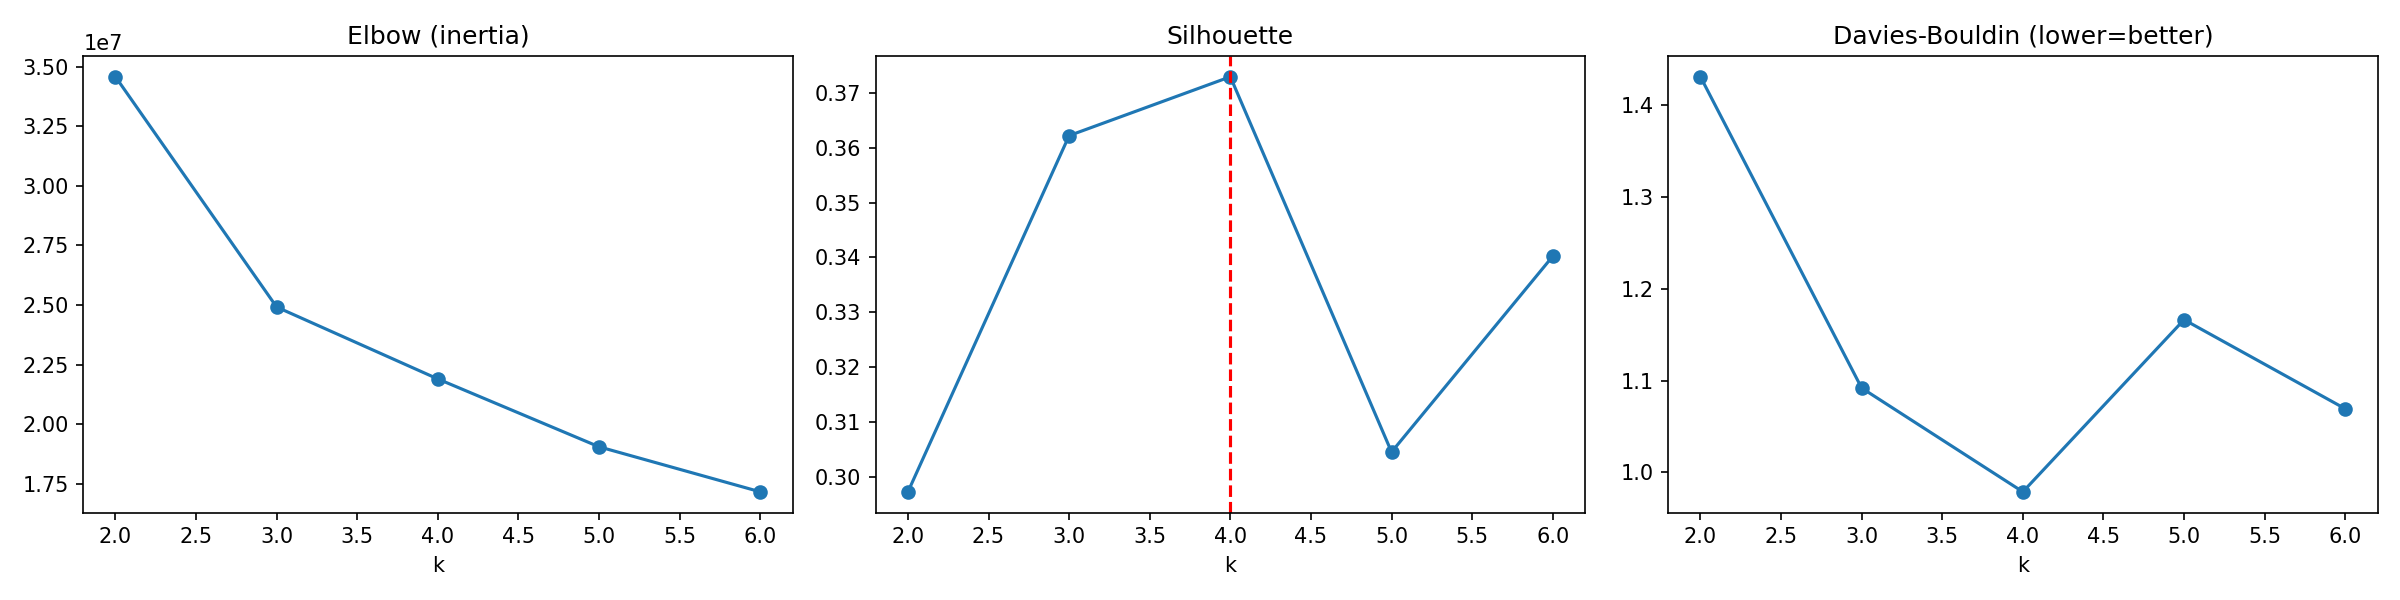
\includegraphics[width=\linewidth]{kmeans_elbow.png}
\caption{Model-order selection.}
\label{fig:kelbow}
\end{subfigure}\hfill
\begin{subfigure}{0.48\textwidth}
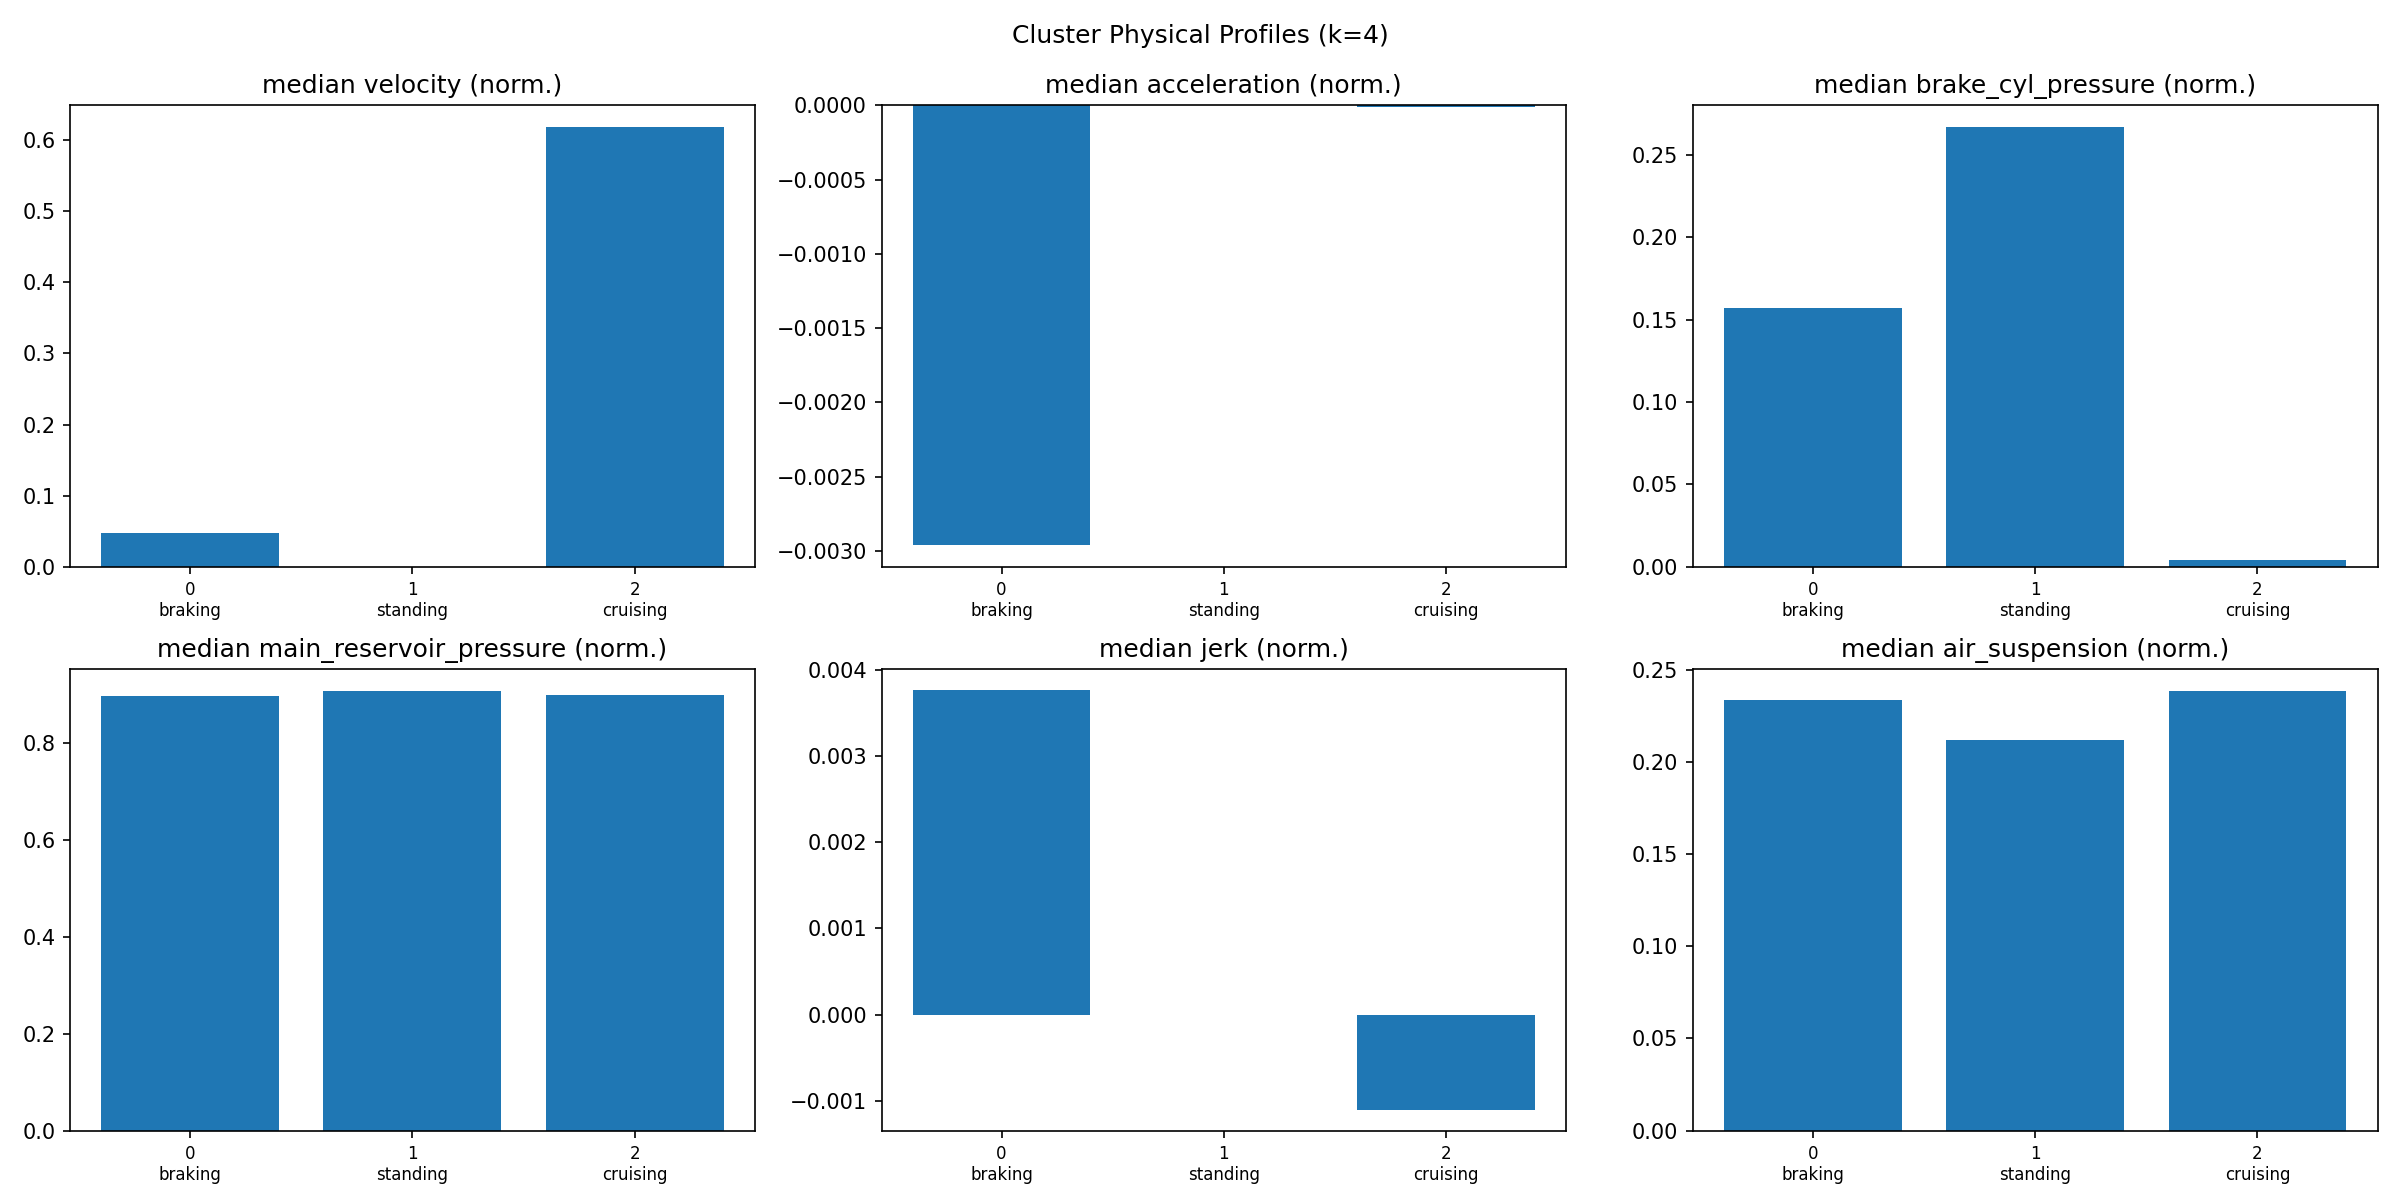
\includegraphics[width=\linewidth]{cluster_profiles.png}
\caption{Per-state median physics.}
\label{fig:profiles}
\end{subfigure}
\caption{Phase~1 clustering. Left: silhouette/Davies--Bouldin across $k$. Right:
physical profile of the three states.}
\end{figure}

\subsubsection*{Transition structure and dwell times}
The row-normalized state-transition matrix (Table~\ref{tab:trans}) and per-state dwell
times (Table~\ref{tab:dwell}) describe the operational rhythm. Standing and cruising are
``sticky'' (self-transition $\approx 0.82$, $0.81$); braking is a short, transitional
state (mean dwell $\approx 11$\,s) that resolves into either standing (0.48) or cruising
(0.43) --- consistent with braking being low-speed deceleration/manoeuvring rather than a
sustained regime.

\begin{table}[H]
\centering
\begin{minipage}{0.52\textwidth}
\centering
\caption{Transition matrix (row-normalized).}
\label{tab:trans}
\small
\begin{tabular}{l r r r}
\toprule
from\,$\backslash$\,to & standing & cruising & braking\\
\midrule
standing & 0.819 & 0.029 & 0.152\\
cruising & 0.003 & 0.814 & 0.182\\
braking & 0.475 & 0.429 & 0.095\\
\bottomrule
\end{tabular}
\end{minipage}\hfill
\begin{minipage}{0.44\textwidth}
\centering
\caption{Dwell times (seconds).}
\label{tab:dwell}
\small
\begin{tabular}{l r r r}
\toprule
State & Mean & Std & Count\\
\midrule
standing & 55.2 & 385.9 & 113{,}106\\
cruising & 53.8 & 20.5 & 117{,}857\\
braking & 11.1 & 3.5 & 210{,}190\\
\bottomrule
\end{tabular}
\end{minipage}
\end{table}

\begin{figure}[H]
\centering

\includegraphics[width=0.62\textwidth]{transition_diagram.png}
\caption{Operational-state transition diagram (training set).}
\label{fig:transdiag}
\end{figure}

\subsection{Results (O2): feature importance}
A random forest trained to recover the cluster label from the window features reaches
\textbf{0.996 test accuracy}, confirming the states are highly separable. The top-ranked
features (Figure~\ref{fig:featimp}) are dominated by \textbf{pneumatic braking force} and
\textbf{proportional-valve pressure} across wagons, with \texttt{TRAIN\_SPEED\_ACTUAL}
entering only at rank~10:
\texttt{MW3/MW1/MW4/MW2\_PNEUMATIC\_BRAKING\_FORCE}, then
\texttt{*\_PROPORTIONAL\_VALVE\_PRESSURE}, then mean speed. The pneumatic brake signals,
not velocity, are what most strongly define the regimes --- an important pointer for
Phase~2 and beyond.

\begin{figure}[H]
\centering
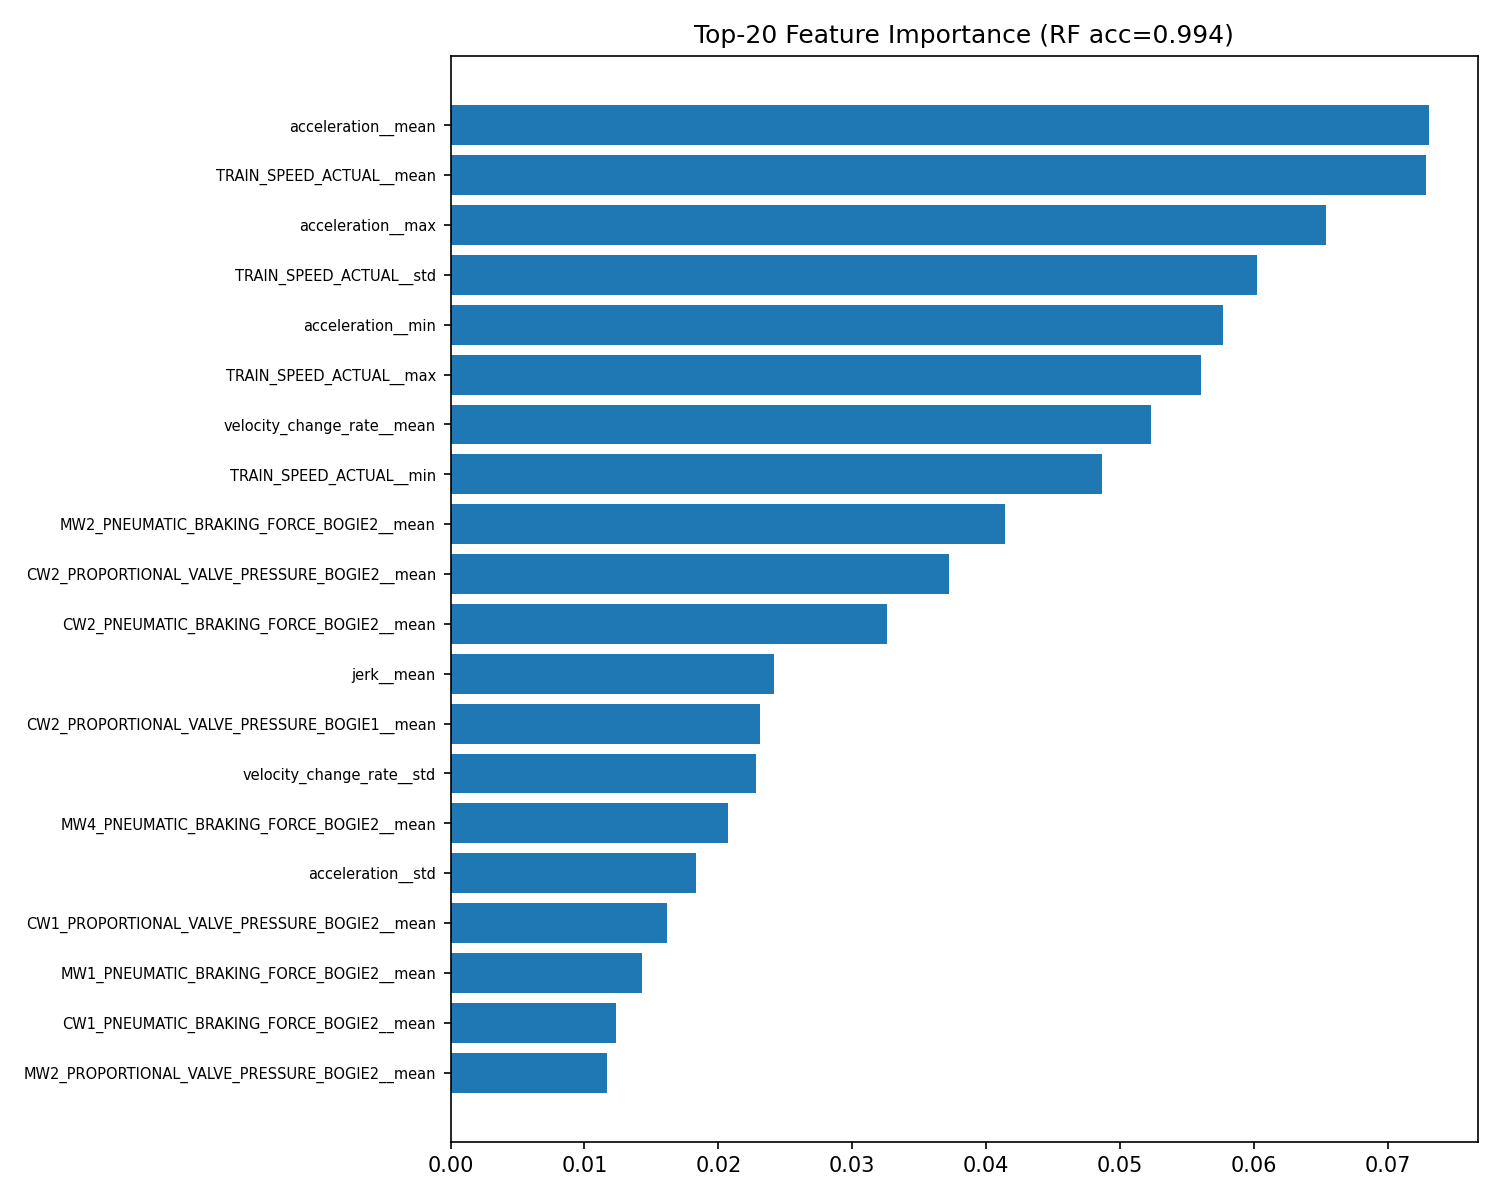
\includegraphics[width=0.7\textwidth]{feature_importance.png}
\caption{Random-forest feature importance for cluster-label recovery (top features).}
\label{fig:featimp}
\end{figure}

\subsection{Validation against documented events (O1)}
For each documented event and several window sizes, the pre-event state distribution was
compared to the baseline distribution by a $\chi^2$ test. Of \textbf{62} tests,
\textbf{60} reject the null at $p<0.05$: the operational-state mix shortly before
documented events differs significantly from normal operation
(Figure~\ref{fig:preevent}). This establishes that the states are not merely a clustering
artefact but carry information aligned with the maintenance/failure record.

\begin{figure}[H]
\centering
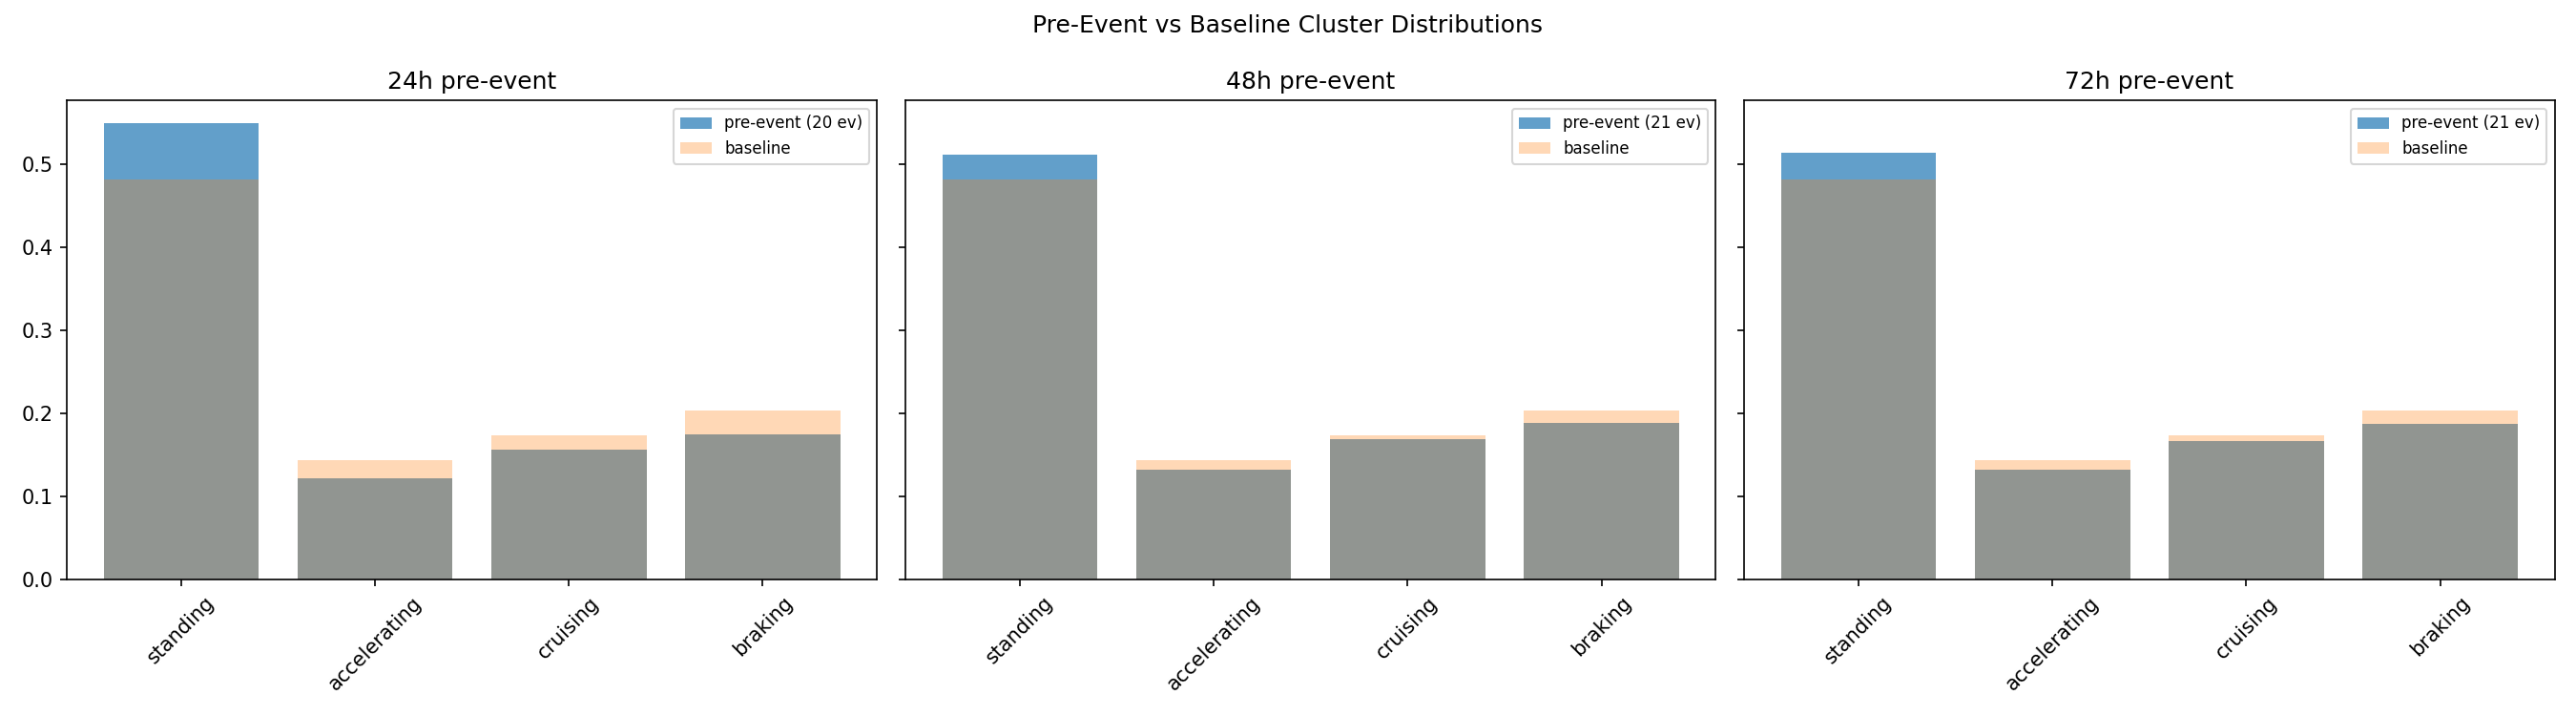
\includegraphics[width=0.7\textwidth]{pre_event_cluster_distributions.png}
\caption{Pre-event vs.\ baseline operational-state distributions.}
\label{fig:preevent}
\end{figure}

\subsection{Critical assessment}
\emph{Learned:} the train genuinely operates in three pneumatically distinct,
overwhelmingly separable regimes, and the ``no accelerating state'' result is a real,
defensible finding rather than a modelling failure. \emph{Guessed (not shown):} RQ1 as
literally phrased asks for regimes that \emph{correlate with wear}; Phase~1 shows the
regimes exist and differ before events, but the wear link itself is asserted, not
demonstrated, until Phase~2. \emph{Needs investigation:} the RF accuracy of 0.996 is
near-circular --- the label \emph{is} a function of these features, so this validates
separability, not predictive value; a cleaner test would predict an external target.
\emph{Unexpected:} braking windows have near-zero net velocity change but the highest
within-window dynamics, i.e.\ ``braking'' is really low-speed manoeuvring, which is why it
is 15.6\,\% of windows yet has the shortest dwell. \emph{Worth asking?} Yes, as
scaffolding --- the states become the unit for everything in Phase~2 --- though RQ1 is only
half answered.

\setcounter{section}{5}
\section{Phase~2 --- Braking Event Analysis}
\label{sec:phase2}

\textit{Realises P2 $\rightarrow$ RQ3/RQ4 $\rightarrow$ O3/O4 of the exposé.}

\subsection{Objective}
Phase~2 takes the windows labelled \emph{braking} by Phase~1, segments them into
individual braking events, quantifies braking stress (RQ3/O3), and tests whether
degradation trends precede the documented brake failures (RQ4/O4).

\subsection{Event extraction}
Contiguous braking windows are merged into discrete events, yielding
\textbf{157{,}823 braking events} over the training period. Per event, features
capturing both the severity and the smoothness of the braking action are extracted:
peak and mean deceleration, duration, a jerk profile, and the brake-cylinder pressure
integral.

\subsection{Intensity classification (O3)}
Because the data are normalized, intensity boundaries are set as \textbf{empirical
quantiles} on peak deceleration rather than physical thresholds
(Table~\ref{tab:intensity}). This yields a roughly \textbf{60\,\% light / 38\,\% heavy /
2\,\% emergency} split. The boundaries are realised as an interpretable decision tree
(Figure~\ref{fig:dtree}) so the category rules remain explainable, and each category's
typical deceleration profile is characterised in Figure~\ref{fig:intprofiles}.

\begin{table}[H]
\centering
\caption{Braking-intensity thresholds on normalized peak deceleration.}
\label{tab:intensity}
\small
\begin{tabular}{l l l r}
\toprule
Category & Rule & Quantile & Fraction\\
\midrule
light & $<0.0448$ & $<$P60 & 0.597\\
heavy & $[0.0448,\,0.0670)$ & P60--P98 & 0.383\\
emergency & $\geq 0.0670$ & $\geq$P98 & 0.020\\
\bottomrule
\end{tabular}
\end{table}

\begin{figure}[H]
\centering
\begin{subfigure}{0.48\textwidth}
\includegraphics[width=\linewidth]{deceleration_distribution.png}
\caption{Peak-deceleration distribution.}
\label{fig:decdist}
\end{subfigure}\hfill
\begin{subfigure}{0.48\textwidth}
\includegraphics[width=\linewidth]{intensity_profiles.png}
\caption{Typical profiles per intensity class.}
\label{fig:intprofiles}
\end{subfigure}
\caption{Braking-intensity characterisation. Boundaries are quantile-based (P60, P98).}
\end{figure}

\begin{figure}[H]
\centering
\includegraphics[width=0.6\textwidth]{decision_tree.png}
\caption{Interpretable decision tree realising the intensity thresholds.}
\label{fig:dtree}
\end{figure}

\subsection{Temporal trends (O4 / RQ3)}
Monthly intensity counts and weekly rolling brake-pressure-integral and jerk-RMS series
were computed over the seasonal coverage 2024-06 to 2025-02
(Figures~\ref{fig:monthly}--\ref{fig:jerk}). These describe the full-year braking-load
profile relevant to maintenance planning.

\begin{figure}[H]
\centering
\includegraphics[width=0.7\textwidth]{monthly_braking_intensity.png}
\caption{Monthly braking-intensity counts (training period).}
\label{fig:monthly}
\end{figure}

\begin{figure}[H]
\centering
\begin{subfigure}{0.48\textwidth}
\includegraphics[width=\linewidth]{brake_pressure_rolling.png}
\caption{Weekly rolling brake-pressure integral.}
\label{fig:brakeroll}
\end{subfigure}\hfill
\begin{subfigure}{0.48\textwidth}
\includegraphics[width=\linewidth]{jerk_rms_rolling.png}
\caption{Weekly rolling jerk-RMS.}
\label{fig:jerk}
\end{subfigure}
\caption{Temporal braking-load series across the training period.}
\end{figure}

\subsection{Pre-failure analysis (RQ4)}
For each of the \textbf{8 documented brake failures}, a 30-day OLS trend was fitted to the
brake-pressure-integral series preceding the flag onset, and a rising precursor was
counted when the slope was positive at $p<0.10$. \textbf{Only 1 of 8} brake failures
shows such a rising precursor (Figure~\ref{fig:precase}). A complementary CUSUM
change-point detector on the weekly pressure-integral series found \textbf{1}
change-point, and that single change-point fell within 30~days before a brake failure
(Figure~\ref{fig:cusum}).

\begin{figure}[H]
\centering
\begin{subfigure}{0.48\textwidth}
\includegraphics[width=\linewidth]{pre_failure_case_studies.png}
\caption{30-day pre-failure trend case studies.}
\label{fig:precase}
\end{subfigure}\hfill
\begin{subfigure}{0.48\textwidth}
\includegraphics[width=\linewidth]{cusum_analysis.png}
\caption{CUSUM change-point detection.}
\label{fig:cusum}
\end{subfigure}
\caption{Pre-failure degradation analysis on the aggregate braking series.}
\end{figure}

Both results are close to what chance would produce, so \textbf{early warning from
single-signal braking trends alone is \emph{not} established}. This is reported as a
preliminary negative finding rather than a predictor.

\subsection{Critical assessment}
\emph{Learned:} braking can be turned into a clean, large, reproducibly labelled event
dataset (157{,}823 events) --- deliverable O3 is solid. \emph{Guessed / weak:} the
degradation claim (RQ4) is barely supported (1/8 precursor trends; 1 relevant CUSUM
change-point), close to chance; honestly reported, but it means aggregate braking trends
are not a reliable early-warning device. \emph{Needs investigation:} the quantile
thresholds (P60/P98) are statistical conveniences --- without physical units or
inspection-confirmed severity, ``emergency'' is a label of convenience; tying intensity to
real wear needs component-inspection data. The pre-failure trend also uses the flag onset
as ground truth, which may lag the true degradation start.
\emph{Unexpected:} how \emph{little} signal precedes failures in the aggregate braking
series --- a useful negative result that directly motivated the multivariate health index
in the later phase. \emph{Worth asking?} Yes, and the answer is informative precisely
\emph{because} it is mostly negative.

\setcounter{section}{6}
\section{Phase~3 --- Deeper Analysis and Failure-Driver Discovery}
\label{sec:phase3}

\textit{An extension beyond the exposé.} Phase~2's weak precursor signal motivated four
follow-up questions: does the regime model \emph{generalise} out-of-sample (Task~A); are
the regimes recoverable from \emph{pneumatics alone} (Task~B); where does the variance and
degradation actually \emph{localise} (Tasks~C, D); and can a \emph{multivariate} detector
or an explicit \emph{forecaster} do better than single-signal braking trends (Tasks~E, F)?
Phase~3 is also the first sanctioned use of the held-out test set.

\subsection{Task A --- Held-out test validation (out-of-sample)}
The frozen Phase-1 scaler/PCA/$k$-means and Phase-2 intensity thresholds were applied,
without refitting, to the test span 12~Feb~--~30~Jun~2025 (811{,}667 windows). The state
mix is stable (Table~\ref{tab:traintest}): the $\chi^2$ statistic is enormous
($8460$, $p\approx0$) only because $N$ is huge, but the \emph{magnitudes} are small
(max $|\Delta|=0.062$). Test-set silhouette is \textbf{0.304}, comparable to train, and
the per-state median physics match closely. Re-extracting braking events on the test set
(74{,}772 events) and applying the \emph{train} thresholds gives a 64.7\,/\,26.2\,/\,9.1
light/heavy/emergency split --- the regime structure and intensity boundaries
\textbf{transfer}. A parity caveat: the train clip-bounds were not persisted, so Task~A
skips clipping (justified by the data already being normalized).

\begin{table}[H]
\centering
\caption{State mix, train vs.\ held-out test. Differences are small in magnitude.}
\label{tab:traintest}
\small
\begin{tabular}{l r r r}
\toprule
State & Train prop. & Test prop. & $|\Delta|$\\
\midrule
standing & 0.419 & 0.380 & 0.039\\
cruising & 0.425 & 0.487 & 0.062\\
braking & 0.156 & 0.133 & 0.023\\
\bottomrule
\end{tabular}
\end{table}

\begin{figure}[H]
\centering
\begin{subfigure}{0.48\textwidth}
\includegraphics[width=\linewidth]{test_state_distribution.png}
\caption{Test-period state distribution.}
\end{subfigure}\hfill
\begin{subfigure}{0.48\textwidth}
\includegraphics[width=\linewidth]{train_test_pressure_continuity.png}
\caption{Brake-pressure series across the train/test boundary.}
\end{subfigure}
\caption{Task~A: the operational-state model and braking series transfer to the
held-out period.}
\end{figure}

\subsection{Task B --- Sensor-only regime recovery (RQ5)}
To test whether the velocity channel does all the work, all 10 velocity-derived window
features were dropped, the remaining 162 sensor features re-standardised, PCA(0.95)
applied (29 components), and $k$-means ($k=3$) re-run. Agreement with the velocity-based
labels is an \textbf{adjusted Rand index of 0.970}: the pneumatic sensors alone recover
the regimes, with cluster purities of 1.00/0.99/0.98 for standing/braking/cruising. This
matters for inference whenever the speed channel cannot be trusted --- though, as a caveat,
the near-perfect ARI partly reflects that brake/valve pressures are \emph{mechanistically}
tied to motion, so it confirms redundancy as much as independent discovery.

\subsection{Task C --- PCA variance attribution (RQ6)}
The Phase-1 PCA keeps 31 components for 95\,\% variance (9 already cover $\sim$80\,\%).
Attributing the captured variance to sensor groups (Table~\ref{tab:pcavar}) shows it is
spread \emph{evenly} across the active brake/valve groups --- proportional valve, spring
brake, pneumatic force, and brake cylinder each carry $\approx$14\,\% --- rather than
concentrated, consistent with the heavy redundancy. The leading components load on
pneumatic braking force (PC1, PC2) and spring-brake pressure (PC3). This is descriptive,
not causal: high variance does not imply failure relevance (Task~F partly contradicts it),
but it tells a degradation monitor where to look first.

\begin{table}[H]
\centering
\caption{Share of captured (95\,\%) variance by sensor group (top groups).}
\label{tab:pcavar}
\small
\begin{tabular}{l r r}
\toprule
Sensor group & \% of captured variance & \# features\\
\midrule
Proportional valve & 14.48 & 24\\
Spring brake & 14.47 & 24\\
Pneumatic braking force & 14.43 & 24\\
Brake cylinder & 14.40 & 24\\
Load pressure & 12.50 & 24\\
Derived & 9.23 & 16\\
Load signal & 6.56 & 12\\
Velocity & 5.84 & 10\\
Energy-braking resistance & 4.69 & 8\\
Main reservoir & 2.32 & 4\\
Ambient temperature & 1.07 & 2\\
\bottomrule
\end{tabular}
\end{table}

\begin{figure}[H]
\centering
\begin{subfigure}{0.48\textwidth}
\includegraphics[width=\linewidth]{pca_variance_by_group.png}
\caption{Variance contribution by sensor group.}
\end{subfigure}\hfill
\begin{subfigure}{0.48\textwidth}
\includegraphics[width=\linewidth]{pca_biplot.png}
\caption{PCA biplot of leading components.}
\end{subfigure}
\caption{Task~C: variance is spread evenly across the active brake/valve groups.}
\end{figure}

\subsection{Task D --- Per-wagon / per-bogie localization (RQ7)}
Two weekly signals were streamed over the 12 brake-cylinder and 12 load-pressure sensors
across 38 weeks: a per-sensor wear proxy (mean during braking windows, with a per-sensor
OLS slope) and rolling correlations of normally-redundant sensor pairs. One sensor,
\texttt{CW1\_BRAKE\_CYLINDER\_PRESSURE\_BOGIE2}, diverges from its group trend
($|z|\approx2.2$). More strikingly, of 13 pair-week decorrelations (weekly $r$ dropping
below 0.9 from a baseline $|r|>0.98$), \textbf{12 cluster in the week of 2024-08-19 --- a
Brake System Failure date}. This is the most concrete result of Phase~3: degradation can
be localized in time and to specific pneumatic pairs, and the decorrelation coincides with
a real failure rather than a maintenance action. Two caveats temper it: a 48-week revision
falls $\sim$8 days later, confounding the failure with a major service, and the
decorrelations are abrupt (one week) rather than a slow drift, arguing for a sudden fault
for that event.

\begin{figure}[H]
\centering
\begin{subfigure}{0.48\textwidth}
\includegraphics[width=\linewidth]{per_wagon_brake_trends.png}
\caption{Per-wagon braking-mean trends.}
\end{subfigure}\hfill
\begin{subfigure}{0.48\textwidth}
\includegraphics[width=\linewidth]{correlation_breakdown_timeline.png}
\caption{Redundant-pair decorrelation timeline.}
\end{subfigure}
\caption{Task~D: decorrelations concentrate in the 2024-08-19 brake-failure week.}
\end{figure}

\subsection{Task E --- Multivariate pneumatic health index (RQ8)}
The unsupervised health index of Section~\ref{sec:method} (PCA reconstruction error +
Mahalanobis distance vs.\ a 30-day healthy reference, CUSUM-thresholded at 3.5 for
$\approx$0 false alarms over the 115 failure-free days) detects \textbf{30\,\% of failures
(3/10)} at a \textbf{15.3-day mean lead time} with \textbf{0 false alarms / 6 months}
(Table~\ref{tab:healthidx}). This beats the single-signal Phase-2 approach ($\sim$1/8) and
gives a real lead time --- the project's best degradation-detection result. It remains
modest: 30\,\% detection is low, the ``healthy reference'' (first 30 clean days) is assumed
not verified, and the false-alarm rate rests on a thin 115-day denominator.

\begin{table}[H]
\centering
\caption{Task~E per-failure detection (alarm within 30 days before onset).}
\label{tab:healthidx}
\small
\begin{tabular}{l l c r}
\toprule
Failure type & Onset & Detected & Lead (days)\\
\midrule
Brake System & 2024-10-10 & yes & 3\\
Compressor Module & 2024-10-31 & yes & 24\\
Brake System & 2025-01-21 & yes & 19\\
\multicolumn{4}{l}{\emph{(7 further failures not detected within the 30-day window)}}\\
\midrule
\multicolumn{2}{l}{\textbf{Overall}} & \textbf{3/10 (30\,\%)} & \textbf{15.3 mean}\\
\bottomrule
\end{tabular}
\end{table}

\begin{figure}[H]
\centering
\begin{subfigure}{0.48\textwidth}
\includegraphics[width=\linewidth]{health_index_timeline.png}
\caption{Daily health index with alarms.}
\end{subfigure}\hfill
\begin{subfigure}{0.48\textwidth}
\includegraphics[width=\linewidth]{health_index_leadtime.png}
\caption{Detection lead times.}
\end{subfigure}
\caption{Task~E: multivariate health index and CUSUM alarms.}
\end{figure}

\subsection{Task F --- Failure prediction and SHAP drivers (RQ9, capstone)}
Daily horizon classification under LOGO-CV (Table~\ref{tab:clf}) reveals a key framing
result: \textbf{$H=30$ is degenerate}. With $\sim$10 failures over 8 months, 73\,\% of days
are ``within 30 days of \emph{some} failure'', so the task is nearly trivial-positive and
ROC-AUC collapses to $\approx$0.51. \textbf{$H=7$ is the usable horizon}: HGB reaches
ROC-AUC~$\approx$0.61 and PR-AUC~0.27 against a 0.21 base rate --- modest but above chance.
On the held-out test set the honest number is the H=7 recall of \textbf{5/12}; the H=30
``12/12'' is the same degeneracy. The top global SHAP drivers
(Table~\ref{tab:shap}) are energy-braking resistance and the \textbf{Task~E health-index
features} (Mahalanobis, reconstruction error), followed by velocity, spring-brake, and
brake-cylinder pressure --- a satisfying internal cross-validation, since Tasks~C, D, E, and
F all point at the same components.

\begin{table}[H]
\centering
\caption{Task~F LOGO-CV metrics. A model beats chance when ROC-AUC$>$0.5 and
PR-AUC$>$base rate.}
\label{tab:clf}
\small
\begin{tabular}{l l c c c c}
\toprule
Horizon & Model & Base rate & ROC-AUC & PR-AUC & Prec.@50\%recall\\
\midrule
7d & HGB & 0.205 & \textbf{0.613} & \textbf{0.267} & 0.309\\
7d & logreg & 0.205 & 0.489 & 0.222 & 0.240\\
30d & HGB & 0.726 & 0.506 & 0.710 & 0.772\\
30d & logreg & 0.726 & 0.438 & 0.700 & 0.726\\
\bottomrule
\end{tabular}
\end{table}

\begin{table}[H]
\centering
\caption{Top global SHAP drivers (H=30d, mean $|$SHAP$|$).}
\label{tab:shap}
\small
\begin{tabular}{l r}
\toprule
Feature & mean $|$SHAP$|$\\
\midrule
Energy-braking-resistance (mean) & 2.838\\
Mahalanobis (mean) & 0.378\\
Velocity (p90) & 0.260\\
Spring-brake (mean) & 0.202\\
Brake-cylinder pressure (p90) & 0.174\\
Main-reservoir pressure (p90) & 0.160\\
Reconstruction error (mean) & 0.129\\
\bottomrule
\end{tabular}
\end{table}

\begin{figure}[H]
\centering
\begin{subfigure}{0.48\textwidth}
\includegraphics[width=\linewidth]{failure_pr_curves.png}
\caption{Precision--recall curves.}
\end{subfigure}\hfill
\begin{subfigure}{0.48\textwidth}
\includegraphics[width=\linewidth]{shap_summary.png}
\caption{SHAP global driver summary.}
\end{subfigure}
\caption{Task~F: a weak-but-real 7-day forecast signal; drivers concentrate in the
health-index and brake/pressure features.}
\end{figure}

\subsection{Critical assessment of Phase~3}
\emph{Learned:} the regimes transfer out-of-sample (Task~A, the single most valuable
result), are latent in the pneumatics (Task~B), degradation can be \emph{localized} and
time-aligned to a real failure (Task~D), a multivariate health index meaningfully
out-performs single-signal trends (Task~E), and there is a weak-but-real 7-day forecast
whose drivers cross-validate the health index (Task~F). \emph{Honest limits:} every
\emph{failure-related} metric rests on $N=10$ flag-derived failures, so AUCs are
directional not precise; the H=30 degeneracy is a framing lesson, not a success; the
healthy reference and CUSUM tuning are small-sample targets; and Task~D's strongest
finding is confounded with a near-simultaneous revision.

\subsection{Verification plan (when failure documentation arrives)}
The capstone is N-limited, and the binding constraint is labelled failure data. The
documented next steps are: (1) \textbf{re-label by mechanism} (root-cause/component) and
re-run Task~F per mechanism; (2) \textbf{validate drivers} --- check SHAP-identified sensors
against the documented failed components (does a Task-D brake-cylinder bogie match the
repaired part?); (3) \textbf{lead-time ground truth} --- convert Task~E lead times from
``first alarm $\rightarrow$ flag'' to ``first alarm $\rightarrow$ true onset'' and recompute
the false-alarm rate against confirmed-healthy periods; (4) \textbf{maintenance
effectiveness} --- correlate pre-maintenance health-index level with maintenance extent;
(5) \textbf{cross-train generalization} --- refit and transfer-test if more trains are
released.

\setcounter{section}{7}
\section{Cross-cutting Discussion}
\label{sec:discussion}

\paragraph{Convergent evidence.}
Four independent analyses point at the same components. Phase~1 feature importance ranks
pneumatic braking force and proportional-valve pressure highest; Task~C attributes the
most variance to exactly those brake/valve groups; Task~D localizes degradation to a
brake-cylinder sensor in the week of a brake failure; and Task~F's SHAP drivers
concentrate in brake-cylinder/pressure features plus the Task~E health index. This
triangulation is reassuring: the signal a maintenance monitor should watch is consistent
across unsupervised clustering, variance attribution, localization, and supervised
forecasting.

\paragraph{Supervised vs.\ unsupervised detection.}
Task~E (an always-on, tunable CUSUM monitor on the health index) and Task~F (a horizon
forecaster) are complementary rather than competing: the health index gives a continuous,
self-calibrating alarm with a real lead time, while the classifier answers the explicit
``failure within $H$ days?'' question. Both rest on the same engineered features, which is
why the health-index scores surface as top SHAP drivers in Task~F.

\paragraph{Operational implications for Wiener Linien.}
What is actionable today is the \emph{method and the descriptive layer}: stable,
transferable operational regimes, a reproducible braking-event dataset, a localizable
degradation signal, and a health index that gives $\sim$15-day warning on a minority of
failures. What is \emph{not} yet actionable is scheduling: one would not plan maintenance
on a 30\,\%-recall, $N=10$ model. The deliverable is a validated pipeline and a clear
statement of what data would make it deployable, not a deployable predictor.

\paragraph{Methodological reflection.}
The strongest aspects are strict streaming/memory discipline, schema-driven code reuse,
frozen-model out-of-sample testing (Task~A), and a consistent refusal to oversell weak
results (Phase~2's 1/8, Task~F's H=30 degeneracy). The recurring weakness is
\textbf{$N=10$}: clustering and description are well-powered (millions of windows), but
every failure-related claim rests on ten flag-derived events on a single train.
Leave-one-failure-out CV is the right tool, but it cannot manufacture statistical power
that is not there. The binding constraint is \emph{labelled failure data}, not method ---
which is itself a useful result, because it names exactly what would unlock real
prediction.

\setcounter{section}{8}
\section{Limitations and Threats to Validity}
\label{sec:limitations}

\begin{itemize}[leftmargin=1.4em,itemsep=0.2em]
\item \textbf{Single train.} All results come from one Wiener Linien vehicle; nothing here
establishes generalisation across rolling stock.
\item \textbf{Normalized, non-physical units.} Min--max normalization removes physical
scale, so the Phase~2 intensity categories (Table~\ref{tab:intensity}) are statistical,
not physical, and ``emergency'' braking is not anchored to a deceleration in m/s$^2$.
\item \textbf{Ten flag-derived failures define $N$.} Every Phase~2 failure-related number
rests on the 10 logical failures (8 brake) produced by the 24\,h flag-merge of
Section~\ref{sec:events}. The merge gap is an unvalidated hyperparameter that sets $N$, and
the flag count was never reconciled against documented incidents.
\item \textbf{Flag-onset timing.} The pre-failure analysis (RQ4) treats the failure flag
onset as the degradation start; if the flag lags true onset, the 30-day window is
mis-aligned and weak precursors could be missed.
\item \textbf{Near-circular Phase~1 validation.} The RF cluster-recovery accuracy of 0.996
validates separability, not external predictive value, because the label is a function of
the input features.
\item \textbf{Compressed seasonality.} Ambient temperature is normalized to a narrow
range, so the seasonal/route load effects the exposé hoped to study are muted in the
training window.
\item \textbf{No repair/material data.} The additional Wiener Linien maintenance data
(duration, extent, material use) were not received, so braking intensity and pre-failure
trends cannot be cross-checked against what was actually repaired.
\item \textbf{Test-set clip-bound parity (Task~A).} Train clip-bounds were not persisted,
so the out-of-sample evaluation skips clipping; justified by the data being normalized,
but a small parity gap remains.
\item \textbf{Small-sample health index (Task~E).} The 30\,\% detection rate, 15.3-day
lead, and 0-false-alarm tuning rest on 10 failures and a 115-day failure-free denominator;
the ``healthy'' reference is assumed, never verified.
\item \textbf{H=30 degeneracy and mixed mechanisms (Task~F).} Failures occur roughly every
2--3 weeks, making the 30-day horizon trivially positive (base rate 0.73); brake, levelling,
and compressor failures are pooled, capping achievable precision, and the H=7 out-of-sample
recall (5/12) is the only metric to read semi-seriously.
\item \textbf{Localization confound (Task~D).} The strongest localization result coincides
with both a brake failure and a near-simultaneous 48-week revision, which cannot be
separated without repair records.
\item \textbf{Possible slow-degradation leakage.} Excluding active failure/maintenance days
controls obvious leakage, but degradation that began before the labelled onset could still
leak signal into ``negative'' days.
\end{itemize}

\setcounter{section}{9}
\section{Conclusion and Future Work}
\label{sec:conclusion}

\subsection{Status of the research questions}
Table~\ref{tab:status} summarises where each research question stands. The
\emph{descriptive} questions are cleanly answered; the \emph{predictive} ones are the right
questions for a maintenance use-case but are limited by the data, not the method.

\begin{table}[H]
\centering
\caption{Status of each research question: supported, partially supported, or not
established.}
\label{tab:status}
\small
\begin{tabular}{l l p{8.6cm}}
\toprule
ID & Status & Basis\\
\midrule
RQ1 & Partially & Three distinct regimes recovered; the \emph{wear} correlation is asserted, not shown.\\
RQ2 & Supported & Pneumatic braking force and proportional-valve pressure rank highest.\\
RQ3 & Supported & 157{,}823 events; reproducible quantile intensity classes.\\
RQ4 & Not established & Only 1/8 brake failures show a rising precursor (near chance).\\
RQ5 & Supported & Pneumatics recover the regimes without velocity (ARI 0.970).\\
RQ6 & Supported & Variance spread evenly across the brake/valve groups ($\approx$14\,\% each).\\
RQ7 & Supported & Degradation localized to a brake-cylinder pair in a real failure week.\\
RQ8 & Partially & Health index detects 30\,\% of failures at 15.3-day lead, 0 false alarms.\\
RQ9 & Partially & Weak-but-real 7-day forecast (ROC-AUC 0.61); H=30 degenerate; N-limited.\\
\bottomrule
\end{tabular}
\end{table}

\subsection{Headline takeaway}
The project establishes four things. The operational regimes are real, are latent in the
pneumatic signals, and \emph{transfer out-of-sample} --- the strongest evidence that the
model is not overfit. Degradation can be \emph{localized} in time and to a specific
component, and the localization coincides with a documented brake failure. A
\emph{multivariate} health index meaningfully out-performs single-signal braking trends,
giving roughly two weeks of warning on a minority of failures. And failure forecasting,
while above chance at a 7-day horizon, is fundamentally limited by the ten flag-derived
failures available on this single train. For Wiener Linien this is not yet an operational
scheduler --- one would not act on a 30\,\%-recall, $N=10$ model --- but it is a validated
pipeline and, importantly, a precise statement of what additional data would unlock real
prediction. That the binding constraint is \emph{labelled failure data}, not method, is
itself a result.

\subsection{Future work}
The highest-value next step is to reconcile the failure \emph{flags} against documented
incidents: the 24\,h merge gap currently \emph{defines} the failure count $N$, and the flag
onset may lag the true degradation start, which shifts every lead-time and precursor number.
Beyond that, the verification plan of Section~\ref{sec:phase3} applies: re-label failures by
mechanism and re-run the forecaster per mechanism; validate the SHAP-identified sensors
against the actually repaired components; convert lead times to a true-onset reference and
recompute the false-alarm rate against confirmed-healthy periods; and correlate
pre-maintenance health-index level with maintenance extent if material/duration data are
released. Finally, recovering physical units would let the intensity classes be anchored to
real deceleration thresholds, and transferring the pipeline to additional trains --- once
released --- would test cross-vehicle generalization and enlarge the failure sample that
currently caps every predictive result.

\setcounter{section}{10}
\section{Reproducibility and Documentation}
\label{sec:repro}

\begin{itemize}[leftmargin=1.4em,itemsep=0.2em]
\item \textbf{Environment.} \texttt{uv} with pinned Python~3.12 and a versioned lockfile
(\texttt{uv.lock}); \texttt{uv sync} reproduces the environment.
\item \textbf{Deterministic execution.} A fixed random seed (42) governs the scaler, PCA,
$k$-means initialisation, and the random forest, so Phase~1 and Phase~2 outputs are
reproducible run to run.
\item \textbf{Ordered, checkpointed scripts.} The pipeline is a sequence of numbered
scripts (00--12): Step~0 profiling $\rightarrow$ Phase~1 clustering/validation
$\rightarrow$ Phase~2 event extraction/intensity/trend analysis $\rightarrow$ Phase~3
held-out validation, sensor-only clustering, PCA attribution, localization, health index,
and failure prediction. Each writes checkpoints so stages are skippable on re-run, and the
Phase~3 scripts reuse the \emph{frozen} Phase-1/2 models rather than refitting. Streaming
per-day I/O keeps peak memory at $\approx$1.5\,GB even on the 14.3\,M-row training set.
\item \textbf{Tests.} A \texttt{pytest} suite (29 tests, 88\,\% line coverage) covers
preprocessing, windowing, the event-merge logic, and the intensity thresholds.
\item \textbf{Provenance of every figure and table.} Step~0 writes to
\texttt{logs/data\_profiling/} (\texttt{schema.json}, \texttt{full\_stats.csv},
\texttt{event\_inventory.csv}, \texttt{data\_quality.csv},
\texttt{high\_correlation\_pairs.csv}). Phase~1 produces
\texttt{cluster\_profiles.csv}, \texttt{kmeans\_k\_selection.csv},
\texttt{transition\_matrix.csv}, \texttt{feature\_importance\_phase1.csv},
\texttt{phase1\_event\_validation.csv}, and \texttt{models/phase1/cluster\_labels.json};
its figures live under \texttt{results/plots/phase1/}. Phase~2 produces
\texttt{intensity\_thresholds.csv}, \texttt{monthly\_braking\_intensity.csv},
\texttt{pre\_failure\_trends.csv}, and \texttt{cusum\_changepoints.csv}, with figures
under \texttt{results/plots/phase2/}. Phase~3 produces
\texttt{train\_vs\_test\_state\_comparison.csv}, \texttt{cluster\_no\_velocity\_vs\_baseline.csv},
\texttt{pca\_variance\_by\_sensor\_group.csv}, \texttt{per\_sensor\_divergence.csv},
\texttt{correlation\_breakdowns.csv}, \texttt{health\_index\_detection.csv},
\texttt{failure\_prediction\_cv\_metrics.csv}, \texttt{failure\_drivers\_shap.csv}, and
\texttt{failure\_prediction\_test\_oos.csv}, plus the frozen models
\texttt{models/phase3/failure\_clf\_\{7d,30d\}.joblib} and figures under
\texttt{results/plots/phase3/}. Every table and figure in this report maps to one of these
artefacts.
\item \textbf{Data access.} The MetroAT dataset is documented at
\url{https://researchdata.tuwien.ac.at/records/9ja0q-bq581}; the analysis pipeline is
maintained in the project repository with a README covering setup, data access, and
reproduction steps.
\end{itemize}

\end{document}
